% 图 62.2 —— 由 `checks/emit_hand.py` 自动拼出（probe 精测 + prims2 图元分解）
%%
% ⚠ 这是**稿子不是成品**：跑 `checks/checkhand.py 62.2` 看指标 + 看叠合图。
%%
%% ⚠ 待核：
%   · 本图 probe 报出阴影族 2 个 —— **本脚本不生成阴影**（要照原书手写）；prims2 的 strokes 里可能含阴影线，核对时留意别画重
%   · 可疑字形 1 项（空心圈 ⊙ 常被认成字母 o）—— 见文件末
%%
\documentclass[12pt]{standalone}
\usepackage{fontspec}
\setsansfont{Arial}
\newfontfamily\mfallback{DejaVu Sans}
\usepackage{tikz}
\begin{document}
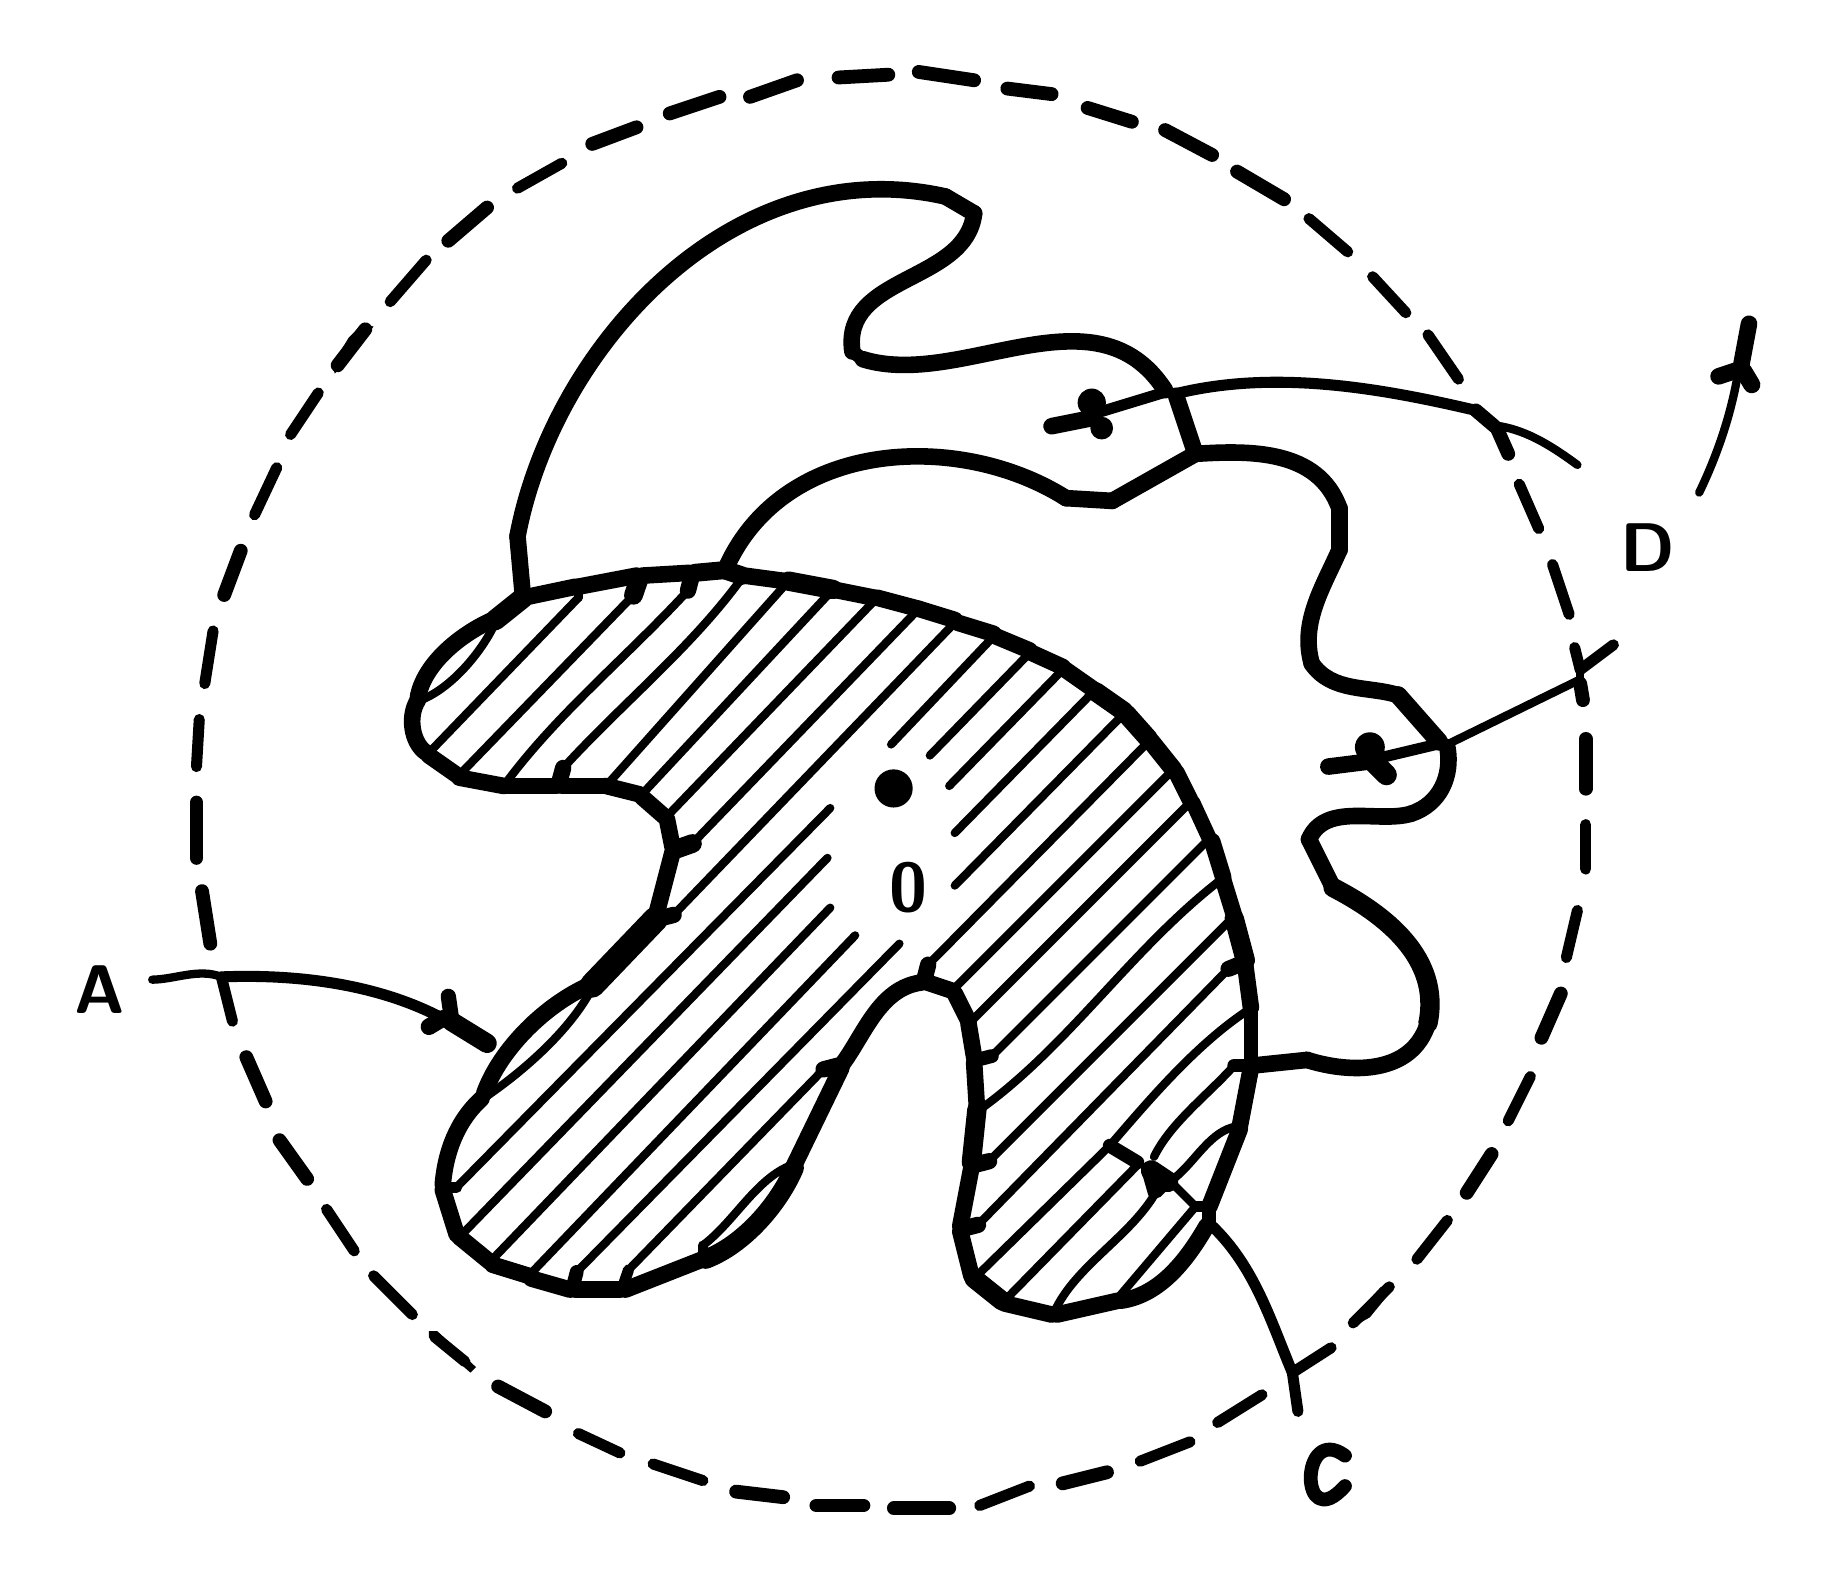
\begin{tikzpicture}[x=1pt, y=-1pt, line width=6.0pt, line cap=round, line join=round]

  %% ════ 填充区（prims2 的 fills）════
  \fill (121.0,107.0) -- (116.0,112.0) -- (110.0,122.0) -- (111.0,125.0) -- (125.0,108.0) -- cycle;
  \fill (494.0,455.0) -- (489.0,455.0) -- (478.0,467.0) -- (478.0,470.0) -- (485.0,466.0) -- cycle;
  \fill (145.0,471.0) -- (145.0,473.0) -- (160.0,486.0) -- (162.0,484.0) -- (148.0,471.0) -- cycle;

  %% ════ 直线段（prims2 的 strokes）════
  \draw[line width=6.0pt] (222.0,198.0) -- (239.0,197.0);
  \draw[line width=4.0pt] (70.0,343.0) -- (74.0,359.0);
  \draw[line width=7.0pt] (386.0,240.0) -- (396.0,247.0);
  \draw[line width=4.5pt] (407.0,421.0) -- (405.0,414.0);
  \draw[line width=5.9pt] (240.0,198.0) -- (238.6,203.4);
  \draw[line width=6.0pt] (611.0,126.0) -- (617.0,124.0);
  \draw[line width=6.0pt] (385.0,239.0) -- (375.0,232.0);
  \draw[line width=4.0pt] (244.0,525.0) -- (226.0,519.0);
  \draw[line width=5.0pt] (86.0,388.0) -- (79.0,372.0);
  \draw[line width=7.0pt] (440.0,337.0) -- (436.0,322.0);
  \draw[line width=3.0pt] (362.0,226.0) -- (326.0,263.0);
  \draw[line width=6.0pt] (385.0,141.0) -- (370.0,144.0);
  \draw[line width=5.0pt] (523.3,138.3) -- (530.0,144.0);
  \draw[line width=6.0pt] (470.0,267.0) -- (486.0,265.0);
  \draw[line width=4.0pt] (61.0,267.0) -- (62.0,250.0);
  \draw[line width=6.0pt] (353.0,461.0) -- (370.0,465.0);
  \draw[line width=6.0pt] (394.0,460.0) -- (372.0,465.0);
  \draw[line width=7.0pt] (166.0,367.0) -- (153.0,359.0);
  \draw[line width=3.0pt] (182.0,450.0) -- (299.0,328.0);
  \draw[line width=4.0pt] (557.0,212.0) -- (551.0,194.0);
  \draw[line width=5.0pt] (437.0,52.0) -- (454.0,62.0);
  \draw[line width=5.0pt] (401.0,410.0) -- (391.0,404.0);
  \draw[line width=4.0pt] (82.0,176.0) -- (90.0,159.0);
  \draw[line width=6.0pt] (145.0,361.0) -- (150.0,358.0);
  \draw[line width=3.0pt] (353.0,460.0) -- (401.0,411.0);
  \draw[line width=5.0pt] (302.0,534.0) -- (285.0,534.0);
  \draw[line width=3.0pt] (157.0,436.0) -- (289.0,300.0);
  \draw[line width=3.0pt] (333.0,274.0) -- (374.0,232.0);
  \draw[line width=7.0pt] (291.0,203.0) -- (275.0,200.0);
  \draw[line width=6.0pt] (291.0,203.0) -- (306.0,206.0);
  \draw[line width=3.0pt] (291.0,203.0) -- (222.0,277.0);
  \draw[line width=5.0pt] (187.0,500.0) -- (170.0,491.0);
  \draw[line width=6.5pt] (510.0,258.0) -- (495.2,241.2);
  \draw[line width=6.0pt] (474.0,188.7) -- (474.0,173.7);
  \draw[line width=4.0pt] (546.0,181.0) -- (539.0,165.0);
  \draw[line width=4.0pt] (477.0,81.0) -- (463.0,69.0);
  \draw[line width=5.0pt] (343.0,373.0) -- (348.4,371.6);
  \draw[line width=3.0pt] (348.4,371.6) -- (426.0,294.0);
  \draw[line width=6.0pt] (230.0,285.0) -- (222.0,278.0);
  \draw[line width=4.0pt] (420.0,511.0) -- (402.0,518.0);
  \draw[line width=5.0pt] (442.0,374.0) -- (442.0,356.0);
  \draw[line width=6.0pt] (436.0,321.0) -- (432.0,308.0);
  \draw[line width=5.0pt] (273.0,531.0) -- (256.0,529.0);
  \draw[line width=6.0pt] (193.0,274.0) -- (209.0,274.0);
  \draw[line width=4.0pt] (64.0,237.0) -- (67.0,218.0);
  \draw[line width=3.0pt] (306.0,207.0) -- (231.0,285.0);
  \draw[line width=5.0pt] (563.0,257.0) -- (563.0,275.0);
  \draw[line width=6.0pt] (420.0,279.0) -- (415.0,269.0);
  \draw[line width=7.0pt] (352.0,460.0) -- (342.0,452.0);
  \draw[line width=6.0pt] (221.0,277.0) -- (209.0,274.0);
  \draw[line width=6.0pt] (179.0,206.0) -- (177.0,183.8);
  \draw[line width=6.0pt] (331.6,61.0) -- (342.0,67.1);
  \draw[line width=4.9pt] (298.0,117.0) -- (301.8,119.8);
  \draw[line width=6.0pt] (179.0,206.0) -- (198.0,202.0);
  \draw[line width=7.5pt] (179.0,206.0) -- (169.0,214.0);
  \draw[line width=5.0pt] (71.0,205.0) -- (77.0,189.0);
  \draw[line width=5.5pt] (421.0,280.0) -- (427.0,293.0);
  \draw[line width=7.0pt] (341.0,410.0) -- (343.0,391.0);
  \draw[line width=5.0pt] (66.0,331.0) -- (63.0,312.0);
  \draw[line width=9.0pt] (204.0,346.0) -- (227.0,322.0);
  \draw[line width=6.0pt] (342.0,372.0) -- (340.0,360.0);
  \draw[line width=5.9pt] (342.0,411.0) -- (347.4,409.6);
  \draw[line width=3.0pt] (347.4,409.6) -- (435.0,322.0);
  \draw[line width=5.0pt] (261.0,25.0) -- (278.0,19.0);
  \draw[line width=7.5pt] (406.0,413.0) -- (412.0,417.0);
  \draw[line width=7.0pt] (405.0,257.0) -- (397.0,248.0);
  \draw[line width=6.5pt] (414.0,268.0) -- (406.0,258.0);
  \draw[line width=6.0pt] (196.0,456.0) -- (182.0,452.0);
  \draw[line width=3.0pt] (335.0,347.0) -- (413.0,269.0);
  \draw[line width=6.0pt] (214.0,456.0) -- (198.0,456.0);
  \draw[line width=6.0pt] (463.0,293.3) -- (471.7,310.7);
  \draw[line width=6.0pt] (462.3,373.0) -- (443.0,375.0);
  \draw[line width=3.0pt] (168.0,445.0) -- (290.0,318.0);
  \draw[line width=3.0pt] (290.0,282.0) -- (155.0,419.0);
  \draw[line width=4.0pt] (155.0,419.0) -- (151.0,419.0);
  \draw[line width=6.0pt] (199.0,202.0) -- (220.0,198.0);
  \draw[line width=4.0pt] (492.0,455.0) -- (479.0,468.0);
  \draw[line width=5.9pt] (228.0,322.0) -- (233.4,320.6);
  \draw[line width=3.0pt] (233.4,320.6) -- (335.0,215.0);
  \draw[line width=3.5pt] (244.0,444.0) -- (244.0,440.0);
  \draw[line width=5.0pt] (436.0,375.0) -- (441.0,375.0);
  \draw[line width=3.0pt] (560.0,236.0) -- (513.0,259.0);
  \draw[line width=6.0pt] (374.0,231.0) -- (363.0,226.0);
  \draw[line width=4.0pt] (446.0,494.0) -- (430.0,504.0);
  \draw[line width=3.0pt] (391.0,404.0) -- (343.0,451.0);
  \draw[line width=5.0pt] (561.0,237.0) -- (562.0,243.0);
  \draw[line width=4.0pt] (177.0,58.0) -- (193.0,49.0);
  \draw[line width=6.0pt] (337.0,433.0) -- (341.0,412.0);
  \draw[line width=5.0pt] (166.0,65.0) -- (152.0,77.0);
  \draw[line width=6.0pt] (233.0,298.0) -- (227.0,321.0);
  \draw[line width=5.0pt] (383.0,29.0) -- (399.0,34.0);
  \draw[line width=6.0pt] (341.0,451.0) -- (337.0,435.0);
  \draw[line width=6.0pt] (277.0,411.0) -- (294.0,376.0);
  \draw[line width=6.0pt] (343.0,390.0) -- (342.0,374.0);
  \draw[line width=6.2pt] (620.0,124.0) -- (623.0,129.0);
  \draw[line width=6.7pt] (258.0,198.0) -- (252.0,196.0);
  \draw[line width=4.0pt] (362.0,527.0) -- (344.0,534.0);
  \draw[line width=5.0pt] (547.0,365.0) -- (554.0,349.0);
  \draw[line width=4.0pt] (517.0,127.0) -- (506.0,111.0);
  \draw[line width=4.0pt] (95.0,147.0) -- (105.0,132.0);
  \draw[line width=6.0pt] (349.0,219.0) -- (336.0,215.0);
  \draw[line width=6.0pt] (145.0,263.0) -- (155.0,270.0);
  \draw[line width=4.0pt] (131.0,99.0) -- (144.0,84.0);
  \draw[line width=6.0pt] (231.0,286.0) -- (233.0,296.0);
  \draw[line width=4.0pt] (108.0,427.0) -- (118.0,442.0);
  \draw[line width=6.0pt] (427.0,426.0) -- (438.0,398.0);
  \draw[line width=4.0pt] (561.0,232.0) -- (559.0,224.0);
  \draw[line width=4.0pt] (561.0,232.0) -- (573.0,223.0);
  \draw[line width=3.0pt] (561.0,232.0) -- (561.0,235.0);
  \draw[line width=3.0pt] (385.0,240.0) -- (335.0,291.0);
  \draw[line width=5.0pt] (370.0,24.0) -- (354.0,22.0);
  \draw[line width=5.9pt] (193.5,267.5) -- (192.0,273.0);
  \draw[line width=3.0pt] (156.0,270.0) -- (218.9,205.1);
  \draw[line width=6.8pt] (218.9,205.1) -- (221.0,199.0);
  \draw[line width=3.0pt] (341.0,359.0) -- (420.0,280.0);
  \draw[line width=4.0pt] (563.0,304.0) -- (563.0,288.0);
  \draw[line width=4.0pt] (502.0,445.0) -- (513.0,431.0);
  \draw[line width=3.0pt] (414.0,418.0) -- (422.0,426.0);
  \draw[line width=5.0pt] (374.0,526.0) -- (390.0,522.0);
  \draw[line width=5.0pt] (411.0,37.0) -- (428.0,46.0);
  \draw[line width=5.0pt] (529.0,407.0) -- (520.0,421.0);
  \draw[line width=4.0pt] (410.0,132.0) -- (387.0,139.0);
  \draw[line width=5.0pt] (197.0,455.0) -- (198.4,449.6);
  \draw[line width=3.0pt] (198.4,449.6) -- (315.0,331.0);
  \draw[line width=4.0pt] (543.0,379.0) -- (535.0,395.0);
  \draw[line width=4.0pt] (199.0,508.0) -- (214.0,515.0);
  \draw[line width=5.9pt] (324.0,344.0) -- (325.4,338.6);
  \draw[line width=3.0pt] (325.4,338.6) -- (405.0,258.0);
  \draw[line width=4.0pt] (412.0,417.0) -- (408.0,421.0);
  \draw[line width=6.0pt] (415.0,133.0) -- (422.0,154.0);
  \draw[line width=6.0pt] (340.0,359.0) -- (335.0,349.0);
  \draw[line width=6.0pt] (181.0,451.0) -- (168.0,447.0);
  \draw[line width=4.0pt] (471.0,477.0) -- (457.0,486.0);
  \draw[line width=5.0pt] (293.0,18.0) -- (311.0,17.0);
  \draw[line width=5.0pt] (61.0,280.0) -- (61.0,300.0);
  \draw[line width=5.0pt] (232.0,31.0) -- (250.0,25.0);
  \draw[line width=6.0pt] (335.0,214.0) -- (322.0,210.0);
  \draw[line width=6.0pt] (155.0,436.0) -- (150.0,420.0);
  \draw[line width=6.0pt] (438.0,397.0) -- (442.0,376.0);
  \draw[line width=7.5pt] (491.0,270.0) -- (486.0,265.0);
  \draw[line width=6.5pt] (241.0,197.0) -- (252.0,196.0);
  \draw[line width=4.0pt] (509.0,259.0) -- (488.0,264.0);
  \draw[line width=6.0pt] (622.0,107.0) -- (619.0,123.0);
  \draw[line width=5.9pt] (293.0,375.0) -- (287.6,376.4);
  \draw[line width=3.0pt] (287.6,376.4) -- (217.1,448.9);
  \draw[line width=4.0pt] (217.1,448.9) -- (215.0,455.0);
  \draw[line width=3.0pt] (199.0,203.0) -- (199.0,206.0);
  \draw[line width=3.0pt] (199.0,206.0) -- (145.0,262.0);
  \draw[line width=5.0pt] (427.0,432.0) -- (427.0,427.0);
  \draw[line width=5.0pt] (112.0,122.0) -- (122.0,109.0);
  \draw[line width=6.0pt] (191.0,274.0) -- (172.0,274.0);
  \draw[line width=5.9pt] (338.0,434.0) -- (343.4,432.6);
  \draw[line width=3.0pt] (343.4,432.6) -- (433.9,340.1);
  \draw[line width=5.8pt] (433.9,340.1) -- (439.0,338.0);
  \draw[line width=3.0pt] (209.0,274.0) -- (274.0,201.0);
  \draw[line width=5.0pt] (342.0,19.0) -- (322.0,16.0);
  \draw[line width=6.0pt] (274.0,200.0) -- (259.0,198.0);
  \draw[line width=6.8pt] (234.0,297.0) -- (240.2,294.8);
  \draw[line width=3.0pt] (240.2,294.8) -- (322.0,210.0);
  \draw[line width=6.0pt] (350.0,220.0) -- (362.0,225.0);
  \draw[line width=3.0pt] (394.0,459.0) -- (422.0,426.0);
  \draw[line width=5.0pt] (535.0,154.0) -- (531.0,145.0);
  \draw[line width=6.0pt] (307.0,206.0) -- (322.0,210.0);
  \draw[line width=4.0pt] (498.0,103.0) -- (486.0,90.0);
  \draw[line width=4.0pt] (556.0,336.0) -- (560.0,319.0);
  \draw[line width=4.0pt] (125.0,451.0) -- (139.0,465.0);
  \draw[line width=5.0pt] (204.0,42.0) -- (220.0,36.0);
  \draw[line width=6.0pt] (172.0,274.0) -- (156.0,271.0);
  \draw[line width=6.0pt] (167.0,446.0) -- (156.0,437.0);
  \draw[line width=6.0pt] (440.0,339.0) -- (442.0,354.0);
  \draw[line width=3.0pt] (349.0,220.0) -- (312.0,259.0);
  \draw[line width=6.0pt] (422.0,154.0) -- (391.9,171.0);
  \draw[line width=6.0pt] (391.9,171.0) -- (375.2,170.0);
  \draw[line width=6.0pt] (216.0,456.0) -- (244.0,445.0);
  \draw[line width=4.0pt] (147.0,473.0) -- (158.0,482.0);
  \draw[line width=6.0pt] (428.0,294.0) -- (432.0,307.0);
  \draw[line width=4.0pt] (422.0,426.0) -- (426.0,426.0);
  \draw[line width=5.0pt] (91.0,402.0) -- (101.0,416.0);
  \draw[line width=6.0pt] (325.0,345.0) -- (334.0,348.0);
  \draw[line width=5.0pt] (333.0,535.0) -- (313.0,535.0);
  \draw[line width=5.5pt] (152.0,350.0) -- (153.0,357.0);
  \draw[line width=3.0pt] (335.0,310.0) -- (396.0,248.0);
  \draw[line width=4.0pt] (457.0,486.0) -- (459.0,500.0);

  %% ════ 曲线（prims2 的 curves —— 三段式，坐标同为 (y,x)）════
  \draw[line width=3.0pt] (70.0,343.0) .. controls (61.9,339.8) and (53.2,343.9) .. (45.0,344.0);
  \draw[line width=4.0pt] (70.0,343.0) .. controls (97.2,341.9) and (126.4,345.5) .. (150.0,358.0);
  \draw[line width=3.0pt] (238.6,203.4) .. controls (216.4,227.5) and (190.9,248.2) .. (172.0,274.0);
  \draw[line width=4.0pt] (416.0,132.0) .. controls (451.5,123.6) and (489.2,130.3) .. (523.3,138.3);
  \draw[line width=6.0pt] (150.0,418.0) .. controls (151.0,406.4) and (155.0,395.2) .. (164.0,387.0);
  \draw[line width=6.0pt] (495.2,241.2) .. controls (484.7,237.8) and (471.4,240.4) .. (464.0,229.8);
  \draw[line width=6.0pt] (464.0,229.8) .. controls (459.7,214.8) and (468.4,201.6) .. (474.0,188.7);
  \draw[line width=6.0pt] (474.0,173.7) .. controls (466.3,152.1) and (441.1,152.8) .. (422.0,154.0);
  \draw[line width=6.0pt] (177.0,183.8) .. controls (189.8,115.6) and (254.8,43.7) .. (331.6,61.0);
  \draw[line width=6.0pt] (342.0,67.1) .. controls (339.1,92.4) and (294.0,89.2) .. (298.0,117.0);
  \draw[line width=6.0pt] (301.8,119.8) .. controls (337.4,130.8) and (386.0,92.4) .. (411.0,131.0);
  \draw[line width=3.0pt] (618.0,125.0) .. controls (615.5,139.9) and (610.5,154.5) .. (604.0,168.0);
  \draw[line width=6.0pt] (513.0,260.0) .. controls (514.9,270.5) and (510.2,280.6) .. (500.0,284.0);
  \draw[line width=6.0pt] (500.0,284.0) .. controls (488.2,287.6) and (469.0,279.6) .. (463.0,293.3);
  \draw[line width=7.0pt] (471.7,310.7) .. controls (489.9,320.1) and (510.9,335.9) .. (506.0,359.7);
  \draw[line width=6.0pt] (506.0,359.7) .. controls (500.2,378.5) and (477.7,377.9) .. (462.3,373.0);
  \draw[line width=3.0pt] (244.0,440.0) .. controls (255.5,431.3) and (263.1,416.0) .. (276.0,411.0);
  \draw[line width=3.0pt] (407.0,408.0) .. controls (413.1,395.6) and (426.2,385.9) .. (436.0,375.0);
  \draw[line width=6.0pt] (203.0,346.0) .. controls (187.3,352.9) and (170.9,368.8) .. (165.0,385.0);
  \draw[line width=3.0pt] (391.0,404.0) .. controls (405.8,386.8) and (422.5,367.2) .. (441.0,355.0);
  \draw[line width=6.0pt] (323.0,345.0) .. controls (307.6,347.0) and (302.3,364.1) .. (294.0,375.0);
  \draw[line width=6.0pt] (168.0,214.0) .. controls (157.0,218.9) and (143.3,229.4) .. (141.0,242.0);
  \draw[line width=3.0pt] (344.0,391.0) .. controls (376.4,367.7) and (399.0,332.7) .. (431.0,308.0);
  \draw[line width=6.0pt] (426.0,433.0) .. controls (419.2,444.8) and (409.4,458.0) .. (395.0,460.0);
  \draw[line width=6.0pt] (144.0,262.0) .. controls (138.7,258.4) and (137.3,248.7) .. (141.0,243.0);
  \draw[line width=3.0pt] (407.0,422.0) .. controls (397.5,437.4) and (378.4,447.8) .. (371.0,464.0);
  \draw[line width=3.0pt] (258.0,199.0) .. controls (239.9,223.9) and (214.8,244.2) .. (193.5,267.5);
  \draw[line width=3.0pt] (142.0,243.0) .. controls (153.1,238.7) and (164.1,225.6) .. (169.0,215.0);
  \draw[line width=3.0pt] (532.0,144.0) .. controls (542.4,145.8) and (551.4,151.7) .. (560.0,158.0);
  \draw[line width=7.0pt] (245.0,445.0) .. controls (258.7,439.8) and (271.4,425.2) .. (277.0,412.0);
  \draw[line width=3.0pt] (204.0,347.0) .. controls (196.3,361.9) and (179.8,376.5) .. (166.0,386.0);
  \draw[line width=3.0pt] (414.0,416.0) .. controls (421.8,410.1) and (427.2,398.5) .. (437.0,397.0);
  \draw[line width=6.0pt] (375.2,170.0) .. controls (336.7,145.6) and (272.6,148.4) .. (252.0,196.0);
  \draw[line width=5.0pt] (476.0,516.0) .. controls (459.6,504.0) and (459.4,545.6) .. (476.0,527.0);
  \draw[line width=4.0pt] (428.0,433.0) .. controls (443.4,447.8) and (449.2,467.4) .. (457.0,486.0);

  %% ════ 实心点 ════
  \fill (312.9,274.9) circle (6.9);
  \fill (384.5,135.5) circle (5.1);
  \fill (388.1,144.7) circle (4.1);
  \fill (485.0,260.0) circle (5.4);

  %% ════ 标签（probe 直接给的 \node 行）════
  %% ⚠ 全部补了 fill=white：文字在最上层，否则与曲线交叉干扰
     \node[anchor=center,inner sep=0pt,fill=white,font=\fontsize{30.4}{38.0}\selectfont] at (585.3,188.0) {\textsf{\textbf{\textit{D}}}};   % box(573,177,21,21)
     \node[anchor=center,inner sep=0pt,fill=white,font=\fontsize{32.3}{40.4}\selectfont] at (318.2,310.8) {\textsf{\textbf{0}}};   % box(308,299,15,23)
     \node[anchor=center,inner sep=0pt,fill=white,font=\fontsize{29.6}{37.0}\selectfont] at (26.2,347.5) {\textsf{\textbf{\textit{A}}}};   % box(14,336,19,22)

  % 钉死画布：否则超出的图元/控制点会把页面撑大，1:1 回比就失准
  \pgfresetboundingbox
  \path[use as bounding box] (0,0) rectangle (638,548);
\end{tikzpicture}
\end{document}

% ⚠ 待核清单（probe 拿不准，人眼过一遍）：
%   · 未识别/跳过：⑤ 跳过/未识别的字形
